\documentclass[a4paper, 12pt]{article}
\usepackage{geometry}
\geometry{a4paper,
	total={170mm,257mm},left=2cm,right=2cm,
	top=1cm,bottom=2cm}

\usepackage{mathtext}
\usepackage{amsfonts} 
\usepackage{amsmath}
\usepackage[T2A]{fontenc}
\usepackage[utf8]{inputenc}
\usepackage[english,russian]{babel}
\usepackage{graphicx, float}
\usepackage{tabularx, colortbl}
\usepackage{caption}
\captionsetup{labelsep=period}

\newcommand{\parag}[1]{\paragraph*{#1:}}
\DeclareSymbolFont{T2Aletters}{T2A}{cmr}{m}{it}
\newcounter{Points}
\setcounter{Points}{1}
\newcommand{\point}{\arabic{Points}. \addtocounter{Points}{1}}
\newcolumntype{C}{>{\centering\arraybackslash}X}

\author{Костылев Влад, Б01-208}
\date{\today}
\title{\textbf{Множества и логика} \\ 
	домашнее задание}

\begin{document}
	\maketitle
	
	%1
	\textbf{№1}\
	\
	$(A \backslash B) \cap ((A \cup B) \ (A \cap B)) \stackrel{?}{=} A \backslash B$
	
	\[
	\text{л.ч. } (a \wedge \overline{b}) \wedge ((a \vee b)\wedge (\overline{a \wedge b})) = (a \wedge \overline{b}) \wedge ((a \vee b) \wedge (\overline{a} \vee \overline{b}))
	\]
	
	\[
	\text{п.ч. } a \wedge \overline{b}
	\]
	
	Если мы возьмем a и b = 0, то вся л.ч. тоже = 0 и п.ч. = 0. Если возьмем a и b отличные от нуля, то л.ч. = п.ч. $\Rightarrow$ л.ч. = п.ч.
	
	%2
	\textbf{№2}\
	\
	$( (A \backslash B) \cup (A \backslash C) ) \cap (A \backslash (B \cap C)) \stackrel{?}{=} A \backslash (B \cup C)$
	
	\[
	\text{л.ч. }
	((a \wedge \overline{b}) \vee (a \wedge \overline{c})) \wedge (a \wedge (\overline{b \wedge c})) = a \wedge (b \vee c) \wedge (\overline{b} \vee \overline{c})
	\]
	
	\[
	\text{п.ч. }
	a \wedge (\overline{b \vee c}) = a \wedge \overline{b} \wedge \overline{c} 
	\]
	
	Если мы возьмем b и c = 0, то вся л.ч. тоже = 0, а правая часть = a $\Rightarrow$ л.ч. $\not=$ п.ч.
	
	%3
	\textbf{№3}\
	\
	$(A \cap B) \backslash C \stackrel{?}{=} (A \backslash C) \cap (B \backslash C)$
	
	\[
	\text{л.ч. }
	a \wedge b \wedge \overline{c}
	\]
	
	\[
	\text{п.ч. }
	a \wedge \overline{c} \wedge b \wedge \overline{c} = a \wedge b \wedge \overline{c} \Rightarrow \text{л.ч. = п.ч}
	\]
	
	%4
	\textbf{№4}\
	\
	$(A \cup B) \backslash (A \backslash B) \subset B$
	
	\[
	(a \vee b) \wedge (\overline{a \wedge \overline{b}}) \rightarrow b = 1
	\]
	
	\[
	\overline{b \vee (a \wedge \overline{a})} \vee b = 1 \Leftrightarrow b \vee \overline{b} = 1 \Rightarrow верно. 
	\]
	
	%5
	\textbf{№5}\
	\
	$P = [10; 40]; Q = [20; 30];$
	$((x \in A) \rightarrow (x \in P)) \wedge ((x \in Q) \rightarrow (x \in A))$ 
	
	\[
	(A \subset P) \wedge (Q \subset A) \Rightarrow A \text{ начинается между $[10; 10]$, и кончается между [30; 40]} 
	\]
	
	\[
	\Rightarrow \text{Максимально возможный отрезок = 30, а минимальный = 10.}   
	\]
	
	%6
	\textbf{№6}\
	\
	$A \cap X = B \cap X; A \cup Y = B \cup Y$ Верно ли $A \cup (Y \backslash X) = B \cup (Y \backslash X)?$
	
	\[
	\text{л.ч:  }
	a \vee (y \wedge \overline{x}) = (a \vee y) \wedge (a \vee \overline{x}) = (b \vee y) \wedge (\overline{x} \vee (a \wedge x)) = (b \vee y) \wedge (\overline{x} \vee (b \wedge x)) = (b \vee y) \wedge (b \vee \overline{x})
	\]
	
	\[
	\text{п.ч:  }
	b \vee (y \wedge \overline{x}) = (b \vee y) \wedge (b \vee \overline{x})
	\]
	
	$\Rightarrow$ л.ч. = п.ч., значит верно.
	
	%8
	\textbf{№8}\
	\
	Возьмем следующие A, B, C и D:
	\begin{figure}[H]
		\centering
		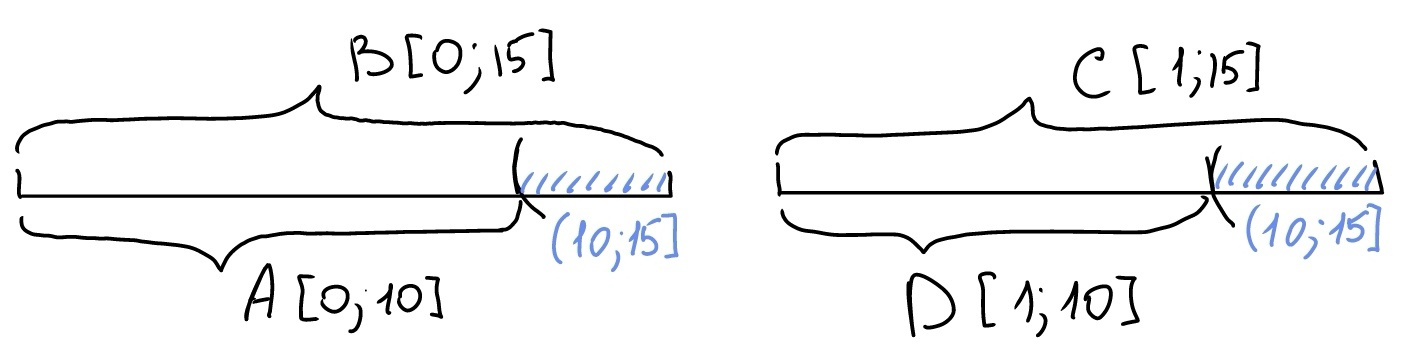
\includegraphics[width=0.6\textwidth]{1}
	\end{figure}
	
	Из рисунка видно, что $A \triangle B = C \triangle D = (10; 15]$
	\[
	A \cap B = A = [0; 10] \Rightarrow [0; 10] \not\subset [1; 15] \Rightarrow \text{неверно.}
	\]
	
\end{document}